\cotefile{80}
\scanpage{3}
\mspage{1}

\diagram{\begin{tikzcd}[ampersand replacement=\&,column sep=small]
\deleted{\substack{C(I)\\ \simeq C_{\mathrm{aff}}(I_0)}}\arrow[r]\arrow[d] \& \deleted{C_{n+1}\simeq C(I)/\mathfrak S_I}\\
\deleted{C_{\mathrm{aff}}(n)\simeq C_{\mathrm{aff}}(I_0)/\mathfrak S_{I_0}\simeq C_{\mathrm{aff}}(I)/\mathfrak S_I} \&
\end{tikzcd}}

\deleted{$I,\ i_0\in I$\quad $\operatorname{Card}I=n+1$\quad $I_0=I-\{i_0\}$}

\margin{Classification pseudo-droites}

\diagram{\resizebox{\linewidth}{!}{\begin{tikzcd}[ampersand replacement=\&,column sep=small,row sep=large]
\substack{C(I)\\ \simeq C_{\mathrm{aff}}(I_0)}
 \arrow[dr,"\substack{\text{oubli du }I\text{-}\text{épinglage}\\ \text{sauf }\Delta_{i_0}=\Delta}","\alpha\,\mathord{/\mkern-5mu/}"'] \& \&\\
\& \substack{C_{\mathrm{aff}}(n)\simeq C_{\mathrm{aff}}(I_0)/\mathfrak S_{I_0}\\
 \simeq C_{\deleted{\unsure{\mathrm{aff}}}}(I)/\mathfrak S_{I_0}}
 \arrow[dl,"\beta"'," \substack{=\ \text{oubli du }\Delta\ \unsure{\text{marquage}|\text{marqué}}\\ \deleted{\unsure{\text{gommage du}|\text{quotienté du}}}\\\text{par }\Delta}"]
 \arrow[dr,"\beta'"',"\substack{=\deleted{\text{oubli du }\Delta}\\\text{gommage}\ \text{du }\Delta}" description] \&\\
 C(n+1)\simeq C(I)/\mathfrak S_I \& \& C(n)
\end{tikzcd}}}

\margin{classes d'iso de systèmes $(X,\Sigma,\Delta)$ où $(X,\Sigma)$ syst. de ps dr et $\Delta\in\Sigma$}

$\beta$ surjective, la fibre en \deleted{\unsure{$(X,$|$X$}} $\mathrm{cl}_{n+1}(X,\Sigma)$ est l'ens. des types d'éléments de $\Sigma$, i.e.

\[
\Sigma/G_{X,\Sigma}
\]

[Si $n=5$, $n+1=6$, il y a deux fibres qui sont de card $1$, deux de card. $2$

$\beta'$ surjective (?) La fibre de $\mathrm{cl}_{n}(X,\Sigma^{*})$ est l'ens des types de positions relatives p.r. à $(X,\Sigma^{*})$

[Si $n=5$, $C(n)$ a un élément, la fibre est de card. \unsure{$6$|$5$}]

\uline{NB}\quad $C_{\mathrm{aff\,st.}}(I_0)\subset C_{\mathrm{aff}}(I_0)$.\quad stable par $\mathfrak S_I$, a fortiori par $\mathfrak S_{I_0}$, passant aux quotients on trouve les diagrammes analogues avec

\[
C_{\mathrm{st}}(I)\quad\text{''}\qquad C\text{''}(I)
\]

\[
C_{\mathrm{st}}(I)=C_{\mathrm{aff\,st}}(I_0),\ C_{\mathrm{aff\,st}}(n),\ C_{\mathrm{st}}(n),\ C_{\mathrm{st}}(n+1).
\]
% archive sheet number: 2
\scanpage{4}
\mspage{2}

Considérons un élément de

\[
 C_{\mathrm{st}}(I)\simeq C_{\mathrm{aff\,st}}(I_0)
\]

$\xi=\mathrm{cl}(X,\Sigma=(\Delta_i)_{i\in I})$. Alors $I_0$ hérite d'une \uline{structure polygonale} \inserted{(dépendant de $\xi$)} (on suppose $\operatorname{card} I_0\geq 3$) De plus, on trouve un polygône $\widetilde I_0(\xi)$ qui est un revêtement à deux feuillets de $I_0(\xi)$. Si on

\diagram{\begin{tikzcd}[ampersand replacement=\&]
\widetilde I_0(\xi)\arrow[d,phantom,"\downarrow" description]\\ I_0(\xi)
\end{tikzcd}}

\deleted{explicite} \inserted{traduit} la structure $(X,\Sigma=(\Delta_i)_{i\in I})$, en mettant à part $\Delta=\Delta_{i_0}$, à l'aide d'un disque $D=\mathrm{Déc}(X,\Delta)$, \deleted{alors} \inserted{et} d'un \uline{système \inserted{stable} de cordes} \inserted{$\widetilde\Sigma$} dans $D=\widetilde X$ indexé par $I_0$, on trouve \deleted{$\widetilde I_0(\xi)\unsure{\simeq}$ ens des sommets sur $\partial D$.}

\[
\begin{aligned}
\widetilde I_0(\xi)&\simeq\text{ens des sommets sur }\partial D=\partial\widetilde X\\
&\qquad\text{(rev. à deux feuillets de }\Delta\text{)}
\end{aligned}
\]

Soit maintenant $S$ un ens. polygonal de \unsure{sommets|sommet|même} d'ordre $2n$, donné une fois pour toutes. On s'intéresse aux structures

\[
\begin{aligned}
&\unsure{\mathfrak s|\text{de}}\qquad\text{syst. stables de cordes }S\text{-épinglés}\\
&\hspace{4em}\text{(mod }S\text{-isom)}
\end{aligned}
\]

soit $\widetilde C_{\mathrm{st}}(S)$ l'ens de ces structures. Posons

\[
\deleted{\unsure{\mathfrak S}}\quad I_0=S/a_S\qquad a_S\ \text{antipodisme de }S
\]

On a une application naturelle

\[
\widetilde C_{\mathrm{st}}(S)\longrightarrow C_{\mathrm{aff\,st}}(I_0)\deleted{\unsure{(I_0)}}
\]

\deleted{dont la fibre en $\xi$ est en corr. 1--1 avec l'ens des \unsure{L}}
% archive sheet number: 3
\scanpage{5}
\mspage{3)}

dont l'image est le sous-ens

\[
\deleted{\unsure{C_{\mathrm{aff\,st}}}}\quad
\overbrace{C_{\mathrm{aff\,st}}(I_0,\pi_0)}^{\inserted{C_{\mathrm{aff\,st}}^{!}(I_0)}}\subset C_{\mathrm{aff\,st}}(I_0)
\]

\unsure{formé|formée} des $\xi$ tels que la structure polygonale correspondante sur $I_0$, soit la structure polygonale $\pi_0$ donnée sur $I_0$, déduite de la structure polygonale de $S$ par passage au \unsure{quotients|quotient}. Donc on a

\[
\widetilde C_{\mathrm{st}}(S)\longrightarrow C_{\mathrm{aff\,st}}^{!}(I_0)
\]

où le ! indique que $I_0$ est muni de $\pi_0$, i.e. qu'on prend $C_{\mathrm{aff\,st}}(I_0,\pi_0)$. La \deleted{\unsure{type|fibre de}} \inserted{fibre de} $\xi\in C_{\mathrm{aff\,st}}^{!}(I_0)$ s'identifie à l'ens des iso polygonaux

\[
S\mathrel{\overset{\sim}{\rule{2.8em}{0.4pt}}}\widetilde I_0(\xi)
\]

qui \deleted{sont} rendent commutatif le triangle

\diagram{\begin{tikzcd}[ampersand replacement=\&,column sep=small]
 S\arrow[rr]\arrow[dr,"\mathrm{can}"']\&\&\widetilde I_0(\xi)\arrow[dl,"\mathrm{can}"]\\
 \& I_0 \&
\end{tikzcd}}

il est de cardinal $2$ ; \uline{on passe de l'un à l'autre par antipodisme}

\deleted{\uline{Ex} $\operatorname{Card} I_0=5$, $C_{\mathrm{aff\,st}}(I_0)\simeq C_{\deleted{\unsure{\mathrm{aff}}}\mathrm{st}}(I_0\amalg\{i_0\})$ se partage en $6$ classes (orbites sous $\mathfrak S_{I_0}$),}
% archive sheet number: 4
\scanpage{6}
\mspage{4)}

\[
D_{I_0}\subset\mathfrak S_{I_0}\ [\subset\mathfrak S_I]
\]

\diagram{\begin{tikzcd}[ampersand replacement=\&]
 C_{\mathrm{aff\,st}}^{!}(I_0)\arrow[dr,"\alpha^!"']\&[-2em]\subset C_{\mathrm{aff\,st}}(I_0)\arrow[d,"\alpha"]\\
 \& C_{\mathrm{aff}}(n)\simeq C_{\mathrm{aff\,st}}^{!}(I_0)/D_{I_0}
\end{tikzcd}}

\margin{\unsure{autm|autom.} de la str. \uline{polygonale} $I_0$}

Soit $\xi^{\unsure{\natural|\sharp|q|4}}\in C_{\mathrm{aff}}(n)$, alors $(\alpha^!)^{-1}(\xi^\natural)$ (resp. $\alpha^{-1}(\xi^\natural)$) est une orbite sous $D_{I_0}$ (resp. sous $\mathfrak S_{I_0}$), et on a sans doute

\[
\alpha^{-1}(\xi^\natural)\xleftarrow{\sim}\deleted{\unsure{\alpha^{!-1}(\xi^\natural)}}\mathfrak S_{I_0}\mathbin{\wedge}_{D_{I_0}}\alpha^{!-1}(\xi^\natural)
\]

d'où

\[
\operatorname{Card}\alpha^{-1}(\xi^\natural)=
\underbrace{\left(\frac{n!}{2n}\right)}_{\substack{\dfrac{(n-1)!}{2}\\=\text{nb de structures}\\\text{polygonales sur}\\|I_0|}}
\mathbin{.}\operatorname{card}\alpha^{!-1}(\xi^\natural)
\]

On a d'autre part, pour

\[
\begin{aligned}
&\xi\in(\alpha^!)^{-1}(\xi^\natural)\\[-2pt]
&\ \shortparallel\\[-2pt]
&\mathrm{cl}^{!}_{\mathrm{aff}}(X,\Sigma=(D_i)_{i\in I_0\amalg\{i_0\}})
\end{aligned}
\]

que le stabilisateur $G_\xi$ de $\xi$ dans $D_{I_0}$ (ou \unsure{encore|même}, dans $\mathfrak S_{I_0}$, c'est kif-kif) est \deleted{égal} \inserted{isom.} à $\operatorname{Aut}(X,\Sigma,\Delta=D_{i_0})$ ; Donc on trouve
% archive sheet number: 5
\scanpage{7}
\mspage{5)}

\[
\operatorname{card}\alpha^{!-1}(\xi^{\unsure{\natural|\sharp|q|4}})=
\frac{\operatorname{card}D_{I_0}}{\operatorname{card}(G_\xi=\operatorname{Aut}(X,\Sigma,\Delta_{\unsure{*|i_0}}))}
=\frac{2n}{\deleted{\unsure{\mathrm{card}}}N(\xi^\natural)}
\]

Passant au composé

\diagram{\begin{tikzcd}[ampersand replacement=\&,row sep=large]
 \widetilde C_{\mathrm{st}}(S)\arrow[d,"\mathrm{deg.}\ 2"]\arrow[dd,bend left=50,"\widetilde\alpha"]\\
 C_{\mathrm{aff\,st}}^{!}(I_0)\arrow[d,"\alpha^!"]\\
 C_{\mathrm{aff}}(n)\simeq\widetilde C_{\mathrm{st}}(S)/D_S\simeq C_{\mathrm{aff\,st}}^{!}(I_0)/D_{I_0}
\end{tikzcd}}

on trouve

\[
\operatorname{card}\widetilde\alpha^{-1}(\xi^\natural)=\frac{4n}{N(\xi^\natural)}
\]

où

\[
N(\xi^\natural)=\operatorname{card}\operatorname{Aut}(X,\Sigma,\Delta)
\]

où

\[
\xi^\natural=\mathrm{cl}_{\mathrm{aff}}(X,\Sigma,\Delta)
\]

\uline{Ex} 1) $n=\operatorname{card}I_0=3$, alors $\operatorname{card}C_{\mathrm{aff}}(3)=1$, et $\operatorname{Aut}(X,\Sigma,\Delta)\simeq\mathfrak S_3$, de card $6$, donc $\widetilde C_{\mathrm{st}}(S)$ consiste en une seule orbite sous $D_{I_0}$, d'ordre $\frac{12}{6}=2$
% archive sheet number: 6
\scanpage{8}
\mspage{6)}

2) $n=4$, $\operatorname{card} C_{\mathrm{aff}}(n)=1$ i.e. $\widetilde C_{\mathrm{st}}(S)$ une seule orbite sous $D_S$. \deleted{\unsure{Cette orbite}} On a $\operatorname{Aut}(X,\Sigma,\Delta)\simeq\mathbb Z/2\mathbb Z$, donc $N(\xi^{\unsure{\natural|\sharp|q|4}})\simeq 2$, et $\operatorname{card}\widetilde C_{\mathrm{st}}(S)=\frac{4n}{2}=8$

3) $n=5$, $\operatorname{card} C_{\mathrm{aff}}(n)=6\ldots$

\noindent\rule{\linewidth}{0.35pt}\par\noindent\rule{\linewidth}{0.35pt}

\uline{Résumé}\qquad $\widetilde C_{\mathrm{st}}(S)\overset{\mathrm{def}}{=}$ classes d'iso. \deleted{de} disques avec syst. \inserted{stable} de cordes, épinglés par le polygône comb. $S$ d'ordre $2n$.

Dépend fonctoriellement du pol. comb. $S$ (pour iso comb.), \deleted{donc} \deleted{\unsure{a}} $D_S$ opère dessus. Si $\widetilde\xi\in\widetilde C_{\mathrm{st}}(S)$, alors ?

\[
\begin{aligned}
\deleted{\operatorname{Aut}}\ (D_S)_{\widetilde\xi}&\simeq\operatorname{Aut}_{\unsure{\mathrm{isot}|\mathrm{ist}}}(D,\widetilde\Sigma)\\
\shortparallel\quad&\qquad\text{(\unsure{en termes|en terme} des}\\[-2pt]
\text{stabilisateur}&\qquad\text{cat. isotopiques)}\\[-2pt]
\text{de }\widetilde\xi\text{ dans }D_S&\simeq\operatorname{Aut}(X,\Sigma,\Delta).
\end{aligned}
\]

(où $(D,\widetilde\Sigma)\longleftrightarrow(X,\Sigma,\Delta)$, et leur classe est $\widetilde\xi$). Enfin on a

\[
\begin{aligned}
\widetilde C_{\mathrm{st}}(S)/D_S&\simeq C_{\mathrm{aff\,st}}(n)\overset{\mathrm{def}}{=}\text{classes d'iso.}\\
&\hspace{9em}\text{de syst stables}\\
&\hspace{9em}(X,\Sigma,\Delta)\\
\widetilde C_{\mathrm{st}}(S)/\{\unsure{1,}a_S\}&\simeq C_{\mathrm{aff\,st}}^{!}(I_0)\deleted{\unsure{\subset}}\inserted{\subset C_{\mathrm{aff\,st}}(I_0)}\quad\text{où } I_0=S/\{1,a_S\}
\end{aligned}
\]
% archive sheet number: 7
\scanpage{10}
% archive sheet number: 9

\figure{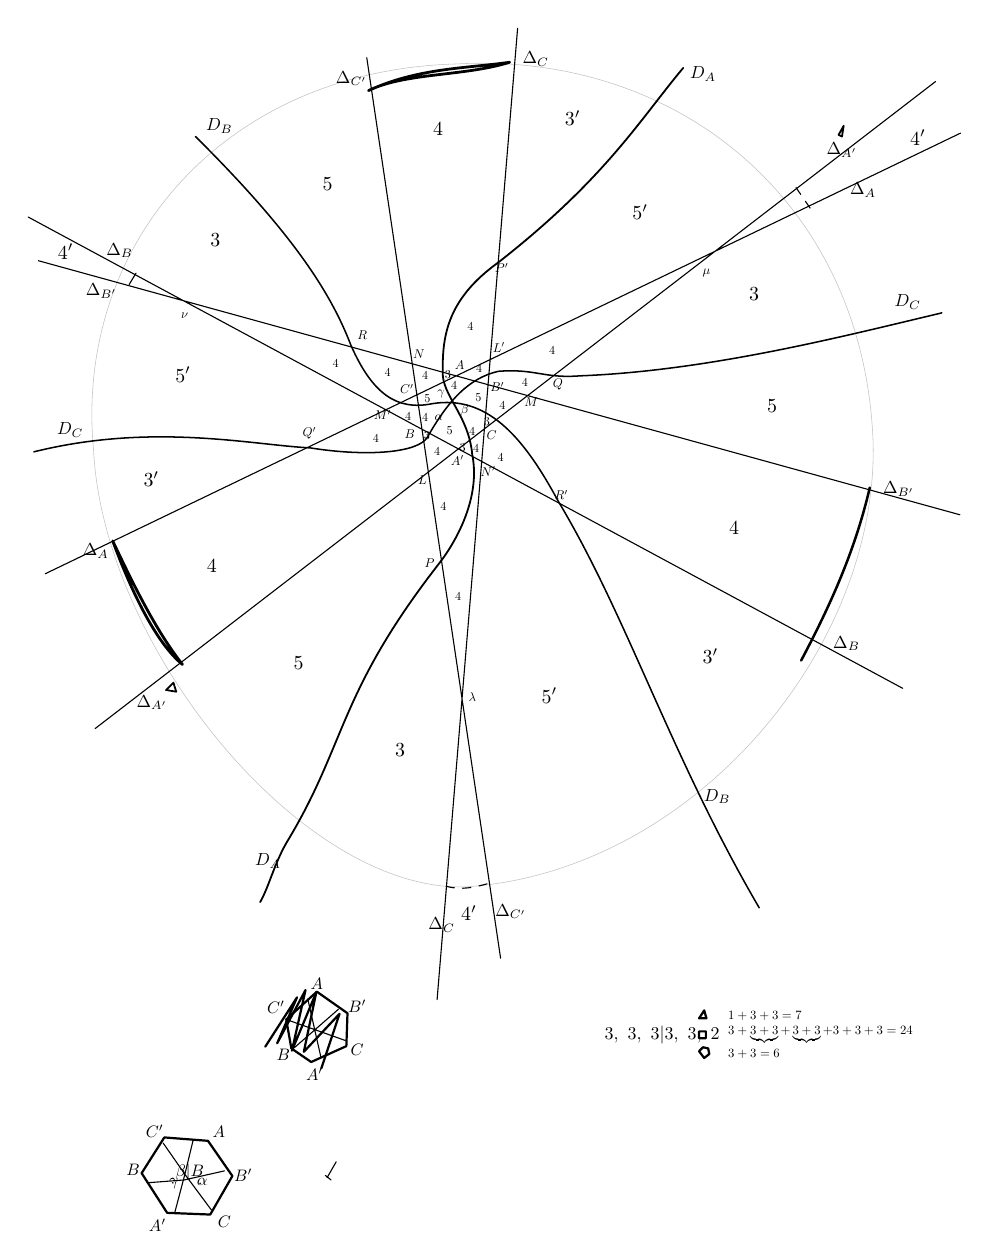
\begin{tikzpicture}[x=.0072cm,y=-.0072cm,line cap=round,line join=round,inner sep=.4pt]
\begin{scope}[shift={(0,0)}]
\draw[gray!48,very thin] (135,766) .. controls (102,404) and (367,99) .. (775,88) .. controls (1171,66) and (1496,337) .. (1510,758) .. controls (1517,1126) and (1188,1512) .. (794,1539) .. controls (505,1551) and (151,1118) .. (135,766);
\draw (20,358)--(1562,1189) (38,435)--(1663,883) (50,987)--(1664,210) (138,1260)--(1620,119) (617,77)--(853,1665) (883,25)--(741,1738);
\draw[line width=.65pt] (1175,95) .. controls (1098,187) and (1038,290) .. (849,438) .. controls (760,502) and (750,566) .. (751,631) .. controls (749,672) and (797,708) .. (803,777) .. controls (818,851) and (776,928) .. (746,967) .. controls (565,1199) and (582,1286) .. (475,1462) .. controls (453,1501) and (444,1540) .. (429,1566);
\draw[line width=.55pt] (315,216) .. controls (481,381) and (552,487) .. (589,584) .. controls (627,670) and (670,700) .. (733,687) .. controls (827,672) and (891,741) .. (954,858) .. controls (1076,1061) and (1153,1309) .. (1309,1576);
\draw[line width=.55pt] (30,772) .. controls (239,720) and (415,760) .. (517,765) .. controls (617,781) and (708,774) .. (724,746) .. controls (761,681) and (797,642) .. (849,630) .. controls (915,625) and (929,643) .. (993,638) .. controls (1222,629) and (1458,568) .. (1631,527);
\draw[line width=1pt] (620,135) .. controls (707,95) and (791,96) .. (869,85) .. controls (790,110) and (685,103) .. (620,135);
\draw[line width=1pt] (169,929) .. controls (200,1014) and (245,1109) .. (292,1147) .. controls (248,1091) and (210,1016) .. (169,929);
\draw[line width=.9pt] (1504,835) .. controls (1477,952) and (1429,1053) .. (1383,1140);
\draw[dashed] (1374,306)--(1400,344) (757,1538) .. controls (784,1546) and (811,1539) .. (832,1533);
\draw (198,477)--(210,457);
\draw[line width=.65pt] (1449,213)--(1458,197)--(1455,216)--cycle (263,1192)--(276,1179)--(281,1195)--cycle;
\node[scale=0.63,transform shape=false] at (590,114) {$\Delta_{C'}$};
\node[scale=0.63,transform shape=false] at (915,79) {$\Delta_C$};
\node[scale=0.63,transform shape=false] at (357,197) {$D_B$};
\node[scale=0.63,transform shape=false] at (1210,106) {$D_A$};
\node[scale=0.63,transform shape=false] at (1455,240) {$\Delta_{A'}$};
\node[scale=0.63,transform shape=false] at (1492,310) {$\Delta_A$};
\node[scale=0.63,transform shape=false] at (1571,508) {$D_C$};
\node[scale=0.63,transform shape=false] at (1555,838) {$\Delta_{B'}$};
\node[scale=0.63,transform shape=false] at (1463,1110) {$\Delta_B$};
\node[scale=0.63,transform shape=false] at (1235,1380) {$D_B$};
\node[scale=0.63,transform shape=false] at (871,1583) {$\Delta_{C'}$};
\node[scale=0.63,transform shape=false] at (749,1607) {$\Delta_C$};
\node[scale=0.63,transform shape=false] at (443,1494) {$D_A$};
\node[scale=0.63,transform shape=false] at (238,1214) {$\Delta_{A'}$};
\node[scale=0.63,transform shape=false] at (139,947) {$\Delta_A$};
\node[scale=0.63,transform shape=false] at (94,734) {$D_C$};
\node[scale=0.63,transform shape=false] at (149,488) {$\Delta_{B'}$};
\node[scale=0.63,transform shape=false] at (181,417) {$\Delta_B$};
\node[scale=0.72,transform shape=false] at (743,202) {$4$};
\node[scale=0.72,transform shape=false] at (980,183) {$3'$};
\node[scale=0.72,transform shape=false] at (1099,349) {$5'$};
\node[scale=0.72,transform shape=false] at (1589,218) {$4'$};
\node[scale=0.72,transform shape=false] at (1300,493) {$3$};
\node[scale=0.72,transform shape=false] at (1332,692) {$5$};
\node[scale=0.72,transform shape=false] at (1265,906) {$4$};
\node[scale=0.72,transform shape=false] at (1223,1132) {$3'$};
\node[scale=0.72,transform shape=false] at (939,1202) {$5'$};
\node[scale=0.72,transform shape=false] at (797,1585) {$4'$};
\node[scale=0.72,transform shape=false] at (676,1298) {$3$};
\node[scale=0.72,transform shape=false] at (497,1145) {$5$};
\node[scale=0.72,transform shape=false] at (344,974) {$4$};
\node[scale=0.72,transform shape=false] at (237,820) {$3'$};
\node[scale=0.72,transform shape=false] at (293,636) {$5'$};
\node[scale=0.72,transform shape=false] at (86,419) {$4'$};
\node[scale=0.72,transform shape=false] at (350,399) {$3$};
\node[scale=0.72,transform shape=false] at (548,299) {$5$};
\node[scale=0.46,transform shape=false] at (855,448) {$P'$};
\node[scale=0.46,transform shape=false] at (1216,457) {$\unsure{\mu}$};
\node[scale=0.46,transform shape=false] at (296,532) {$\unsure{\nu}$};
\node[scale=0.46,transform shape=false] at (803,1204) {$\unsure{\lambda}$};
\node[scale=0.46,transform shape=false] at (728,968) {$P$};
\node[scale=0.46,transform shape=false] at (609,567) {$R$};
\node[scale=0.46,transform shape=false] at (709,599) {$N$};
\node[scale=0.46,transform shape=false] at (781,620) {$A$};
\node[scale=0.46,transform shape=false] at (850,588) {$L'$};
\node[scale=0.46,transform shape=false] at (954,653) {$Q$};
\node[scale=0.46,transform shape=false] at (907,685) {$M$};
\node[scale=0.46,transform shape=false] at (960,848) {$R'$};
\node[scale=0.46,transform shape=false] at (831,807) {$N'$};
\node[scale=0.46,transform shape=false] at (777,787) {$A'$};
\node[scale=0.46,transform shape=false] at (715,822) {$L$};
\node[scale=0.46,transform shape=false] at (516,739) {$Q'$};
\node[scale=0.46,transform shape=false] at (645,707) {$M'$};
\node[scale=0.46,transform shape=false] at (693,740) {$B$};
\node[scale=0.46,transform shape=false] at (837,743) {$C$};
\node[scale=0.46,transform shape=false] at (847,658) {$B'$};
\node[scale=0.46,transform shape=false] at (688,661) {$C'$};
\node[scale=0.46,transform shape=false] at (790,699) {$\unsure{\beta}$};
\node[scale=0.46,transform shape=false] at (744,712) {$\unsure{\alpha}$};
\node[scale=0.46,transform shape=false] at (748,670) {$\unsure{\gamma}$};
\node[scale=0.44,transform shape=false] at (562,617) {$4$};
\node[scale=0.44,transform shape=false] at (654,633) {$4$};
\node[scale=0.44,transform shape=false] at (720,637) {$4$};
\node[scale=0.44,transform shape=false] at (800,552) {$4$};
\node[scale=0.44,transform shape=false] at (944,593) {$4$};
\node[scale=0.44,transform shape=false] at (815,626) {$4$};
\node[scale=0.44,transform shape=false] at (760,636) {$3$};
\node[scale=0.44,transform shape=false] at (771,655) {$4$};
\node[scale=0.44,transform shape=false] at (724,678) {$5$};
\node[scale=0.44,transform shape=false] at (814,677) {$5$};
\node[scale=0.44,transform shape=false] at (896,649) {$4$};
\node[scale=0.44,transform shape=false] at (856,690) {$4$};
\node[scale=0.44,transform shape=false] at (829,719) {$3$};
\node[scale=0.44,transform shape=false] at (803,736) {$4$};
\node[scale=0.44,transform shape=false] at (763,735) {$5$};
\node[scale=0.44,transform shape=false] at (720,712) {$4$};
\node[scale=0.44,transform shape=false] at (690,709) {$4$};
\node[scale=0.44,transform shape=false] at (633,748) {$4$};
\node[scale=0.44,transform shape=false] at (723,743) {$3$};
\node[scale=0.44,transform shape=false] at (741,771) {$4$};
\node[scale=0.44,transform shape=false] at (786,765) {$3$};
\node[scale=0.44,transform shape=false] at (810,766) {$4$};
\node[scale=0.44,transform shape=false] at (853,783) {$4$};
\node[scale=0.44,transform shape=false] at (752,868) {$4$};
\node[scale=0.44,transform shape=false] at (778,1028) {$4$};
\end{scope}
\begin{scope}[shift={(455,1710)}]
\draw[thick] (20,63)--(74,14)--(128,52)--(126,110)--(64,138)--(29,114)--cycle;
\draw (20,63)--(124,100) (34,113)--(112,45) (58,27)--(81,129);
\draw[line width=.8pt] (-17,111)--(39,24)--(4,105)--(54,11)--(30,118)--(73,15)--(51,120)--(114,53)--(82,149);
\node[scale=0.6,transform shape=false] at (74,1) {$A$};
\node[scale=0.6,transform shape=false] at (145,39) {$B'$};
\node[scale=0.6,transform shape=false] at (145,117) {$C$};
\node[scale=0.6,transform shape=false] at (70,159) {$A'$};
\node[scale=0.6,transform shape=false] at (15,126) {$B$};
\node[scale=0.6,transform shape=false] at (2,42) {$C'$};
\end{scope}
\begin{scope}[shift={(1203,1759)}]
\draw[thick] (0,12)--(9,-2)--(13,12)--cycle (0,35) rectangle (12,47) (0,70)--(7,63)--(16,65)--(18,75)--(9,82)--cycle;
\node[scale=.46,anchor=west,transform shape=false] at (50,8) {$1+3+3=7$};
\node[scale=.46,anchor=west,transform shape=false] at (50,42) {$3+\underbrace{3+3}+\underbrace{3+3}+3+3+3=24$};
\node[scale=.46,anchor=west,transform shape=false] at (50,74) {$3+3=6$};
\node[scale=0.65,transform shape=false] at (-65,41) {$\deleted{\unsure{3,\ 3,\ 3|3,\ 3,\ 2}}$};
\end{scope}
\begin{scope}[shift={(205,1969)}]
\draw[thick] (15,75)--(55,12)--(132,18)--(175,80)--(136,148)--(60,145)--cycle;
\draw (53,22)--(92,78)--(138,140) (106,16)--(91,78)--(73,146) (25,92)--(90,87)--(161,71);
\fill (90,76) circle (1.6) (70,92) circle (1.6) (118,93) circle (1.6);
\draw[thin] (342,83)--(358,55) (339,79)--(349,87);
\node[scale=0.6,transform shape=false] at (38,1) {$C'$};
\node[scale=0.6,transform shape=false] at (151,3) {$A$};
\node[scale=0.6,transform shape=false] at (194,79) {$B'$};
\node[scale=0.6,transform shape=false] at (161,161) {$C$};
\node[scale=0.6,transform shape=false] at (43,167) {$A'$};
\node[scale=0.6,transform shape=false] at (0,69) {$B$};
\node[scale=0.6,transform shape=false] at (100,74) {$\unsure{\beta|B}$};
\node[scale=0.6,transform shape=false] at (122,91) {$\unsure{\alpha}$};
\node[scale=0.6,transform shape=false] at (72,94) {$\unsure{\gamma}$};
\end{scope}
\end{tikzpicture}}
% crop-candidate: scan 10
\scanpage{11}
% archive sheet number: 10

Donc si $\widetilde Z'\mathrel{\overset{\sim}{\unsure{\longrightarrow|\rule{1.6em}{0.4pt}}}}X'$ i.e. $Z'\to X'$ est \uline{\unsure{Steinien|steinien}} $\exists!\ \deleted{Z}X'\to\widetilde Z$ \inserted{\uline{$X$-morphisme}} tel que

\diagram{\begin{tikzcd}[ampersand replacement=\&,row sep=small]
 Z\arrow[d]\arrow[dr,phantom,"\mathrm{comm.}"]\&Z'\arrow[l]\arrow[d]\\
 \widetilde Z\arrow[d,dashrightarrow,"\deleted{\unsure{\mathrm{can}}}"']\&X'\arrow[l]\arrow[dl]\\
 \deleted{X}\&
\end{tikzcd}}

En d'autres termes, dans la catégorie des flèches \uline{steiniennes} $Z'\to X'$ \deleted{de $\mathrm{Top}_{/X}$} au dessus de $Z\to X$ il y a un objet initial, savoir $(Z\to\widetilde Z)$ au dessus de $(Z\to X)$

\begin{center}\rule{0.16\linewidth}{0.4pt}\end{center}
Compatibilité \unsure{avec|aux} chgt de base

Quand peut-on \unsure{dire,|dire que} quand

\diagram{\begin{tikzcd}[ampersand replacement=\&,row sep=small]
Z\arrow[d]\&Z'\arrow[l]\arrow[d]\\ X\&X'\arrow[l]
\end{tikzcd}}

est cartésien, que le carré inférieur (ou les deux) de

\diagram{\begin{tikzcd}[ampersand replacement=\&,row sep=small]
Z\arrow[d]\&Z'\arrow[l]\arrow[d]\\
\widetilde Z\arrow[d]\&\widetilde Z'\arrow[l]\arrow[d]\\
X\&X'\arrow[l]
\end{tikzcd}}

le sont ?

a) $Z\to X$ \unsure{comp. et|compact|comp. st} ?

b) $X'\to X$ loc. $\unsure{0|O|\mathcal O}$-acyclique \quad ---
\scanpage{12}
% archive sheet number: 11

\figure{\begin{tikzpicture}[x=.0116cm,y=-.0116cm,line cap=round,line join=round,inner sep=.4pt]
% Drawing 1
\begin{scope}
\draw[gray] (125,257) .. controls (145,152) and (211,115) .. (280,122) .. controls (366,120) and (412,174) .. (400,269) .. controls (375,342) and (326,404) .. (236,416) .. controls (158,400) and (111,347) .. (125,257);
\draw[gray!60] (124,255) .. controls (165,205) and (356,189) .. (410,267) .. controls (375,327) and (175,340) .. (124,255);
\draw[gray!70] (257,129) .. controls (211,178) and (152,400) .. (234,413) .. controls (302,392) and (337,152) .. (261,147);
\draw[gray!45] (263,131) .. controls (209,224) and (182,445) .. (249,390);
\foreach \x/\y in {125/255,195/309,305/220,257/131,236/414,398/272,409/269}{\fill[gray] (\x,\y) circle (3);}
\end{scope}
% Drawing 2
\begin{scope}
\draw[gray] (810,252)--(778,450)--(714,547)--(650,629) (714,547)--(720,619) (714,547)--(778,617)
(778,450)--(830,520)--(809,607) (830,520)--(869,596) (830,520)--(927,588)
(810,252)--(838,452)--(828,482) (838,452)--(878,460) (810,252)--(911,417)--(915,444) (911,417)--(948,421);
\foreach \x/\y in {828/482,878/460,915/438,949/419}{\draw[gray] (\x,\y)--++(-4,13) (\x,\y)--++(14,7) (\x,\y)--++(20,-1);}
\draw[gray!65] (698,646)..controls(731,679)and(723,707)..(737,703)..controls(755,706)and(760,737)..(778,733)..controls(812,706)and(826,744)..(851,750);
\node[scale=0.78,transform shape=false] at (878,723) {$3\times2\times3$};
\end{scope}
% Drawing 3
\begin{scope}
\draw[gray] (423,361)--(566,448)--(523,530)--(344,682)--(306,531)--cycle;
\draw (307,531)--(356,465)--(424,361) (354,466)..controls (402,465) and (446,448)..(470,450)..controls(500,451)and(523,492)..(546,498);
\draw[gray!65] (424,361)--(523,530) (306,531)..controls(378,542)and(476,541)..(520,531);
\draw[thin,dashed,gray] (354,465)--(363,425)--(566,448) (344,682)--(352,579)--(516,536);
\fill (434,354) circle (2.5);
\end{scope}
% Drawing 4
\begin{scope}
\draw[gray!55] (71,860)--(228,575) (162,967)--(332,606) (64,724)--(291,892) (142,598)--(358,776);
\fill[gray] (195,643) circle (5) (215,837) circle (5);
\foreach \x/\y in {121/768,274/715}{\draw (\x-10,\y)--(\x+10,\y) (\x,\y-10)--(\x,\y+10);}
\draw[line width=1pt] (237,984)--(401,723)--(575,842)--(376,1127)--cycle (237,984)--(461,966)--(401,723) (461,966)--(376,1127) (461,966)--(575,842);
\draw[gray,line width=.8pt] (310,854)--(430,848)--(355,973)--(310,854) (330,1089)--(355,973) (310,854)--(381,795)--(508,910) (430,848)--(495,794)--(470,855) (355,973)--(418,1044);
\draw[gray!60] (238,984)--(301,925)--(310,854) (301,925)--(326,955) (355,973)--(375,1127) (363,1007)--(434,1002) (465,851)--(575,842);
\node[scale=0.78,transform shape=false] at (519,721) {$\unsure{\frac43|4\,3|\mathfrak S}$};
\end{scope}
% Drawing 5
\begin{scope}
\draw[gray!45] (667,1371)--(932,1364)--(930,1091)--(676,1090)--cycle (738,1314)--(1005,1302)--(1003,1028)--(742,1027)--cycle (667,1371)--(738,1314) (932,1364)--(1005,1302) (930,1091)--(1003,1028) (676,1090)--(742,1027) (734,1080)--(720,1325) (791,1049)--(796,1214)--(781,1281) (673,1250)--(1005,1243) (678,1147)--(934,1157);
\draw[thick] (669,1244)--(699,1079)--(866,1028)--(968,1091)--(1008,1153)--(979,1297)--(798,1367)--cycle (699,1079)--(808,1141)--(969,1091)--(931,1233)--(798,1367) (669,1244)--(808,1141)--(931,1233)--(979,1297);
\draw (785,1054)--(894,1115)--(868,1344) (667,1244)--(721,1320)--(798,1367) (908,1061)--(947,1099);
\draw[dashed] (699,1079)--(741,1185)--(721,1320)--(849,1252)--(932,1233)--(1008,1153) (741,1185)--(796,1214)--(850,1253) (850,1253)--(979,1297);
\draw[densely dotted,thick] (760,1110)--(792,1106)--(820,1105)--(895,1114)--(909,1066)--(951,1097);
\foreach \x/\y in {699/1079,669/1244,808/1141,931/1233,798/1367,979/1297,968/1091,1008/1153,741/1185,796/1214}{\fill (\x,\y) circle (2.5);}
\foreach \x/\y in {743/1162,767/1134,803/1141,814/1147,740/1183,752/1190,749/1292,770/1320,826/1160,837/1168}{\draw (\x-4,\y+3)--(\x+4,\y-4);}
\node[scale=0.55,transform shape=false] at (709,1198) {$\unsure{3}$};
\node[scale=0.55,transform shape=false] at (834,1317) {$\unsure{4}$};
\end{scope}
% Drawing 6
\begin{scope}
\draw[gray!55] (177,1274)--(355,1254)--(357,1400)--(189,1420)--cycle (209,1235)--(379,1216)--(392,1354)--(218,1374)--cycle (262,1190)--(420,1162)--(420,1301)--(263,1320)--cycle;
\draw[gray!55] (177,1274)--(262,1190) (355,1254)--(420,1162) (357,1400)--(420,1301) (189,1420)--(263,1320) (181,1349)--(353,1325)--(417,1234) (263,1271)--(378,1216)--(355,1325)--(269,1414);
\draw[gray,thick] (268,1414)--(261,1271)--(337,1175);
\draw[gray] (261,1271)--(399,1353) (269,1414)--(355,1325);
\end{scope}
\node at (719,177) {\parbox{2.8cm}{\[\begin{aligned}48&=2.4!\\ \frac{5!}{2.4!}&=\frac{5}{\unsure{2|?}}\end{aligned}\]}};
\node[rotate=17] at (941,854) {\parbox{2.8cm}{\[12=\frac{8\times3\times2}{4}\]}};
\end{tikzpicture}}
% crop-candidate: scan 12
\scanpage{13}
% archive sheet number: 12

\figure{\begin{tikzpicture}[x=0.014cm,y=-0.014cm,line cap=round,line join=round,inner sep=0.4pt]
\draw[gray!80] (261,307)..controls(285,364)and(342,409)..(366,452)..controls(414,546)and(464,583)..(501,660)..controls(529,721)and(551,765)..(578,813);
\draw[gray!75] (241,385)..controls(300,415)and(344,431)..(393,451)..controls(447,472)and(490,520)..(571,544)..controls(613,566)and(666,608)..(696,610);
\draw[gray!80] (294,765)..controls(333,697)and(343,651)..(373,607)..controls(464,494)and(494,427)..(566,297);
\draw[gray!65] (499,307)..controls(499,440)and(506,591)..(504,660)--(511,848);
\draw[gray!80] (230,720)..controls(323,651)and(412,609)..(469,585)..controls(546,557)and(605,519)..(710,514);
\draw[gray!45] (359,639)--(503,527)--(470,586);
\draw[gray!18] (511,847)--(687,724)--(846,983)--(623,966)--cycle (623,966)--(587,1109);
\draw (259,262)--(265,246) (283,292)--(297,246);
\node[scale=0.76,transform shape=false] at (254,351) {$4_2$};
\node[scale=0.76,transform shape=false] at (440,394) {$4_5$};
\node[scale=0.76,transform shape=false] at (537,296) {$4_1$};
\node[scale=0.76,transform shape=false] at (602,449) {$4_3$};
\node[scale=0.76,transform shape=false] at (688,563) {$\unsure{4_6|4_4}$};
\node[scale=0.76,transform shape=false] at (606,667) {$4_2$};
\node[scale=0.76,transform shape=false] at (541,818) {$4_5$};
\node[scale=0.76,transform shape=false] at (411,736) {$4_1$};
\node[scale=0.76,transform shape=false] at (233,767) {$4_3$};
\node[scale=0.76,transform shape=false] at (309,556) {$4_6$};
\node[scale=0.76,transform shape=false] at (419,505) {$3$};
\node[scale=0.76,transform shape=false] at (485,487) {$3$};
\node[scale=0.76,transform shape=false] at (468,544) {$5$};
\node[scale=0.76,transform shape=false] at (521,549) {$3$};
\node[scale=0.76,transform shape=false] at (414,591) {$3$};
\node[scale=0.76,transform shape=false] at (480,613) {$3$};
\end{tikzpicture}}
\scanpage{14}
% archive sheet number: 13

\figure{\begin{tikzpicture}[x=.0074cm,y=-.0074cm,line cap=round,line join=round,inner sep=.4pt]
% Drawing 1
\begin{scope}
\draw (161,41)--(241,115)--(428,177) (239,115)--(496,211) (230,117)--(305,205) (259,129)--(304,173);
\draw[thick] (319,192)--(434,188)--(490,178)--(495,353)--(327,365)--cycle (319,225)--(441,361);
\draw (321,286)--(413,279)--(408,193) (434,188)--(499,213);
\draw[dashed] (319,224)--(491,208) (435,190)--(443,363) (235,119)--(494,348);
\node[scale=0.65,transform shape=false] at (341,177) {$\unsure{-1,+1|-1,-1|-1}$};
\node[scale=0.65,transform shape=false] at (494,165) {$\unsure{1,1|+1}$};
\end{scope}
% Drawing 2
\begin{scope}
\draw[thick] (904,34)..controls(1012,103)and(1260,265)..(1375,375)--(1411,411);
\draw (918,37)--(1021,134) (927,49)--(1086,151) (1096,115)--(1103,360) (1017,214)--(1118,220)--(1241,223) (1220,224)--(1257,374)--(1262,467) (1106,378)--(1234,385)--(1375,376);
\draw (1101,259)--(1218,373) (1099,253)--(1181,361)--(1181,383) (1242,231)--(1240,267) (1230,263)--(1232,384) (1257,379)--(1326,449);
\draw[dashed] (935,51)--(1256,382)--(1324,450) (1100,260)--(1241,260) (1173,260)--(1181,383);
\draw[gray!45] (1093,321)--(1256,316);
\end{scope}
% Drawing 3
\begin{scope}
\draw (263,432)--(1046,971) (326,726)--(1662,879) (351,739)--(408,734)--(1241,733) (441,877)--(1519,890)--(1662,898) (538,471)--(755,1170) (763,426)--(752,1170);
\draw[gray] (630,521)--(616,1138) (792,383)--(594,1135);
\draw[dashed] (508,491)..controls(578,526)and(608,595)..(617,731);
\draw[gray,dash pattern=on 11pt off 8pt] (390,476)--(944,1095);
\node[scale=0.59,transform shape=false] at (578,511) {$Q$};
\node[scale=0.59,transform shape=false] at (783,503) {$R$};
\node[scale=0.59,transform shape=false] at (583,663) {$\unsure{K}$};
\node[scale=0.59,transform shape=false] at (611,650) {$Q'$};
\node[scale=0.59,transform shape=false] at (645,669) {$M'$};
\node[scale=0.59,transform shape=false] at (404,720) {$P$};
\node[scale=0.59,transform shape=false] at (601,739) {$L$};
\node[scale=0.59,transform shape=false] at (631,726) {$B$};
\node[scale=0.59,transform shape=false] at (642,747) {$a$};
\node[scale=0.59,transform shape=false] at (673,737) {$b$};
\node[scale=0.59,transform shape=false] at (717,721) {$C'$};
\node[scale=0.59,transform shape=false] at (777,718) {$N$};
\node[scale=0.59,transform shape=false] at (607,778) {$A'$};
\node[scale=0.59,transform shape=false] at (779,762) {$A$};
\node[scale=0.59,transform shape=false] at (776,834) {$a'$};
\node[scale=0.59,transform shape=false] at (708,876) {$b'$};
\node[scale=0.59,transform shape=false] at (601,897) {$N'$};
\node[scale=0.59,transform shape=false] at (655,898) {$C$};
\node[scale=0.59,transform shape=false] at (774,903) {$B'$};
\node[scale=0.59,transform shape=false] at (906,906) {$L'$};
\node[scale=0.59,transform shape=false] at (597,1041) {$R'$};
\node[scale=0.59,transform shape=false] at (776,1144) {$M$};
\node[scale=0.59,transform shape=false] at (1637,918) {$P'$};
\node[scale=0.59,transform shape=false] at (188,891) {$\unsure{\lambda}$};
\end{scope}
\node at (699,211) {\deleted{\unsure{$N$}}};
\node at (1361,678) {\parbox{4.45cm}{\[
\begin{aligned}
a+a'&<2\\
b+b'&>2\\
2-a'&< b\qquad\text{i.e. }a'+b>2\\
&\qquad(\text{d'où }b>a)
\end{aligned}
\]}};
\end{tikzpicture}}
\scanpage{15}
% archive sheet number: 14

\figure{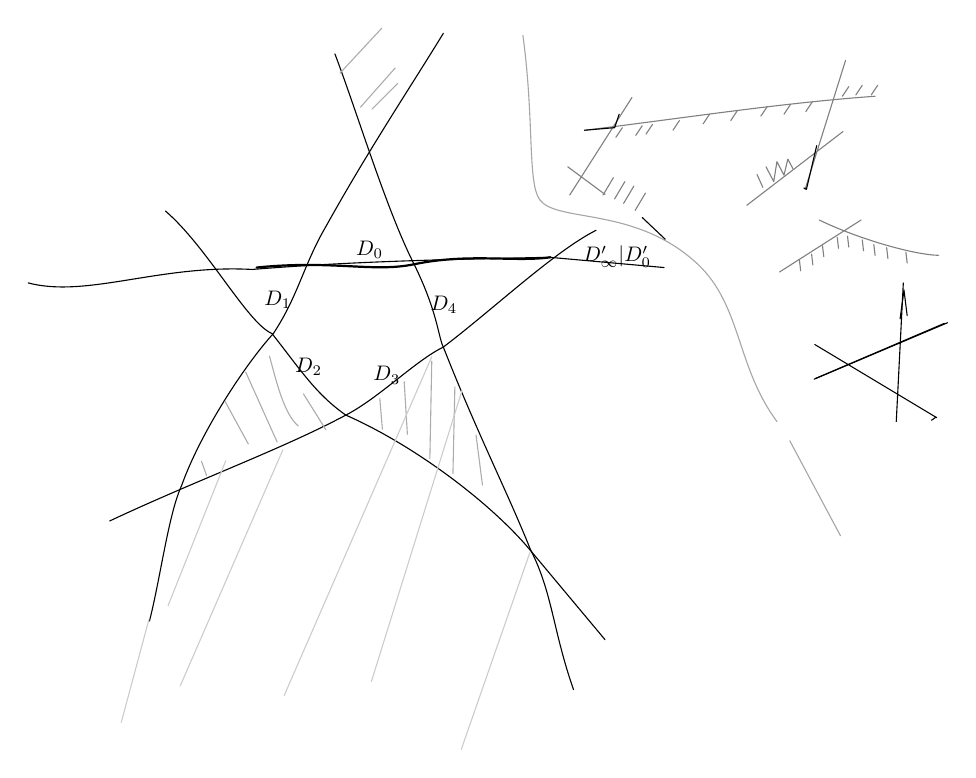
\begin{tikzpicture}[x=.00815cm,y=-.00815cm,line cap=round,line join=round,inner sep=.4pt]
% Drawing 1
\begin{scope}
\draw (212,426)..controls(303,450)and(417,397)..(561,405)..controls(733,391)and(897,389)..(1024,386)--(1203,402);
\draw[thick] (568,402)..controls(686,390)and(750,410)..(813,397)..controls(899,379)and(970,394)..(1026,386);
\draw (401,953)..controls(418,886)and(431,785)..(451,742)..controls(481,658)and(551,552)..(594,505)..controls(633,446)and(641,398)..(676,338)..controls(744,216)and(807,122)..(859,37);
\draw (426,314)..controls(492,371)and(553,488)..(592,505)..controls(637,562)and(660,599)..(707,632)..controls(814,679)and(933,769)..(994,842)--(1111,982);
\draw (339,797)..controls(480,731)and(608,685)..(709,631)..controls(760,604)and(816,547)..(859,526)..controls(938,466)and(1032,377)..(1097,344);
\draw (690,69)..controls(725,161)and(769,308)..(812,394)..controls(850,470)and(851,510)..(859,526)..controls(913,663)and(959,752)..(995,842)..controls(1029,908)and(1030,969)..(1062,1060);
\draw[gray!65] (698,99)--(763,29) (730,152)--(784,91) (748,155)--(788,115) (519,611)--(555,677) (551,565)--(600,674) (588,540)..controls(598,576)and(610,630)..(633,649) (641,599)--(676,655) (482,704)--(490,726) (760,606)--(764,654) (798,580)--(803,662) (841,548)--(838,700) (877,588)--(874,723) (910,663)--(920,741);
\draw[gray!40] (400,951)--(357,1111) (520,703)--(430,929) (609,686)--(449,1054) (841,541)--(611,1069) (888,594)--(747,1047) (994,846)--(887,1153);
\draw[gray!70] (983,40)..controls(1001,171)and(990,269)..(1009,296)..controls(1035,332)and(1152,307)..(1248,390)..controls(1325,455)and(1313,553)..(1379,642) (1399,672)--(1478,820);
\draw (1169,324)--(1205,358);
\node[scale=0.76,transform shape=false] at (744,374) {$D_0$};
\node[scale=0.76,transform shape=false] at (601,452) {$D_1$};
\node[scale=0.76,transform shape=false] at (649,557) {$D_2$};
\node[scale=0.76,transform shape=false] at (771,570) {$D_3$};
\node[scale=0.76,transform shape=false] at (860,460) {$D_4$};
\node[scale=0.76,transform shape=false] at (1130,385) {$\deleted{\unsure{D_{\infty}'|D_0'}}$};
\end{scope}
% Drawing 2
\begin{scope}
\draw[gray] (1080,188)..controls(1249,167)and(1382,146)..(1532,135) (1053,245)--(1111,288) (1056,289)--(1153,137) (1332,305)--(1482,190) (1423,280)--(1486,79);
\draw (1079,188)--(1126,184)--(1133,163) (1421,278)--(1425,280)--(1441,212);
\foreach \x/\y in {1138/184,1169/181,1185/179,1227/173,1274/163,1317/158,1364/151,1400/148,1434/144,1491/120,1512/118,1536/118}{\draw[gray] (\x,\y)--++(-10,15);}
\foreach \x/\y in {1108/289,1126/295,1140/302,1158/313}{\draw[gray] (\x,\y)--++(16,-27);}
\draw[gray] (1348,257)--(1357,277) (1362,245)--(1374,268)--(1379,237)--(1390,258)--(1396,233)--(1404,248);
\draw[gray] (1383,409)--(1510,328) (1445,328)..controls(1505,357)and(1591,382)..(1631,383);
\foreach \x/\y in {1414/390,1433/381,1450/368,1473/355,1489/353,1512/359,1530/366,1550/371,1580/378}{\draw[gray] (\x,\y)--++(2,17);}
\draw (1437,576)--(1645,488) (1438,522)--(1628,636) (1565,642)--(1576,426);
\draw (1439,575)--(1640,489) (1571,482)--(1577,437)--(1582,477) (1620,640)--(1627,635);
\end{scope}

\end{tikzpicture}}
\scanpage{17}
% archive sheet number: 16

Système d'hyperplans (projectifs) réels

% slanted
\margin{Théorie analogue dans le cas affine mais qui revient au cas projectif, \unsure{avec|où} un des $H_i$ \unsure{distingués|distingué}.}

Soit $V$ espace vectoriel réel, $H$ un hyperplan de $V$, on note $D_H$ \inserted{$\subset\mathcal P(V)$} l'ens des trois éléments \deleted{de} $\{H,V'_H,V''_H\}$, où $V'_H$ et $V''_H$ sont les deux demi-espaces ouverts de $V$ déterminés par $H$ ; \deleted{qui forment} alors \deleted{\unsure{$H, V'_+$}} $D_H$ est une partition de $V$ par des ens convexes.

Comme c'est un ensemble à trois éléments, un élément distingué \deleted{$\{$}$H$\deleted{$\}$}, on peut regarder $D_H$ comme un espace vectoriel sur $\mathbb F_3=\{-1,0,1\}$. On a une application canonique

\deleted{\unsure{Soit $V_i$|Soit $V\setminus$}}

\[
\varphi_H:\underset{\substack{\shortparallel\\ V^*/\mathbb R^{*+}}}{\mathbb S}\xrightarrow{\deleted{\varphi_H}}D_H
\]

Soit $(H_i)_{\unsure{i|j|I}\in I}$ une famille finie d'hyperplans de $V$, \uline{distincts}, et considérons l'application

% slanted
\margin{``distincts'' inutile, mais on ne \unsure{gagne} rien essentiellement}

\[
\varphi:S\longrightarrow\prod D_{H_i}=E
\]

définie par les $\varphi_{H_i}$. Les fibres non vides de $\varphi$ forment une partition de $S$ par des \deleted{\unsure{sous}} ens ``convexes'' (i.e. l'image inverse dans $V^*$, \unsure{augm. de} $\{0\}$, est \deleted{convexe} \inserted{un} cône convexe) \uline{\unsure{donc|des|dans}} \uline{connexes} : \inserted{les ``cellules ouvertes''.} Soit

% slanted
\margin{``\unsure{demi convexe|demi-convexe|donc connexes|convexes}'' inutile, sauf lorsque le cône convexe en question est une droite, -- mais si $\bigcap H_i=\{0\}$, ceci n'est pas possible. On supposera \unsure{désormais|donc} $\bigcap H_i=\{0\}$.}

\[
\Sigma\deleted{\unsure{\Sigma}}=\varphi(S)\subset E
\]

l'ens. d'indices de cette partition. C'est une partie de $E$ stable par \inserted{l'} homothétie $-1$ ($-\mathrm{id}_E$), qui correspond au passage \deleted{\unsure{inverse}} d'une fibre

\[
Z^*_{-\alpha}=-Z^*_\alpha\qquad\text{pour }\alpha\in\Sigma
\]

On se propose de déterminer $\overline{Z^*_\alpha}$ pour $i\in I$.
\scanpage{18}
% archive sheet number: 17

% slanted
\margin{\deleted{\unsure{c'est ici que|c'est} le fait que les $H_i$ soient distincts est \unsure{essentiel|inessentiel}}}

On trouve que c'est l'intersection des $\tfrac12$ espaces \uline{fermés} $\overline{V'_{H_i}}=V'_{H_i}\cup H_i$, $\overline{V''_{H_i}}=V''_{H_i}\cup H_i$, déterminés par les $H_i$ ($i\in I$), \inserted{qui contiennent \unsure{$Z_i$|$Z$},} en d'autres termes

\[
\overline{Z^*_\alpha}=\bigcup_{\substack{\beta\in\Sigma\\\text{tel que }i\in I\\\text{implique }k_i(\beta)\leq k_i(\alpha)\\\deleted{\unsure{\sim}}}}Z^*_\beta
=\bigcup_{\substack{\beta\in\Sigma\\\beta\leq\alpha}}Z^*_\beta
\]

où les \deleted{\unsure{$k_i$}}

\[
k_i:E\longrightarrow\deleted{E}D_{H_i}\qquad(i\in I)
\]

sont les fonctions coordonnées, et où on introduit dans $\deleted{E}D_{H_i}$ la relation d'ordre $\leq$ donnée par

\diagram{\begin{tikzcd}[ampersand replacement=\&,column sep=tiny,row sep=small]
\unsure{a'_i|a'|\alpha'_i}\arrow[dr]\&\&\unsure{a''_i|a''|\alpha''_i}\arrow[dl]\\
\&0\&
\end{tikzcd}}

$a',a''$ les deux \unsure{élémts|éléments} $\ne 0$ de $D_{\unsure{H_i|H}}$

i.e. Si $x,y\in D_{H_i}$ on a $x\leq y$ sss $x=0$ ou $x=y$, et on met sur $E=\prod_{i\in I}D_{\unsure{I|i}}$ l'ordre produit.

On \deleted{est alors} met sur $\Sigma$ l'ordre induit, d'où une ``top. inférieure'' sur $\Sigma$, dont les fermés sont les parties \inserted{$A$} de $\Sigma$ telles que $\alpha\in A,\ \beta\leq\alpha\Rightarrow\beta\in A$. On a donc

\[
\beta\leq\alpha\iff\beta\in\overline{\{\alpha\}},\qquad\text{et}
\]

\[
\overline{Z^*_\alpha}=Z^*_{\overline{\{\alpha\}}}
\]

en posant, pour $A\subset\Sigma$

\[
Z^*_A=\bigcup_{\alpha\in A}Z^*_\alpha\ .
\]
\scanpage{19}
% archive sheet number: 18

Plus généralement, on a

\[
\begin{aligned}
\overline{Z^*_A}&=Z^*_{\overline A}\\
\left(\ \bigcup_{\alpha\in A}\overset{\shortparallel}{\overline{Z_\alpha}}=\bigcup_{\deleted{\unsure{\beta}}\alpha\in A}Z_{\overline{\{\alpha\}}}
=Z_{\underbrace{\bigcup_{\alpha\in A}\overline{\{\alpha\}}}_{\overline A}}\ \right)&
\end{aligned}
\]

L'ens \deleted{$\Sigma$} ordonné $\Sigma$ est \deleted{donc un} \inserted{donc} l'ens d'indices d'une stratification \inserted{(finie)} de la sphère $S$, satisfaisant l'axiome de fidélité \inserted{et de} densité \deleted{(toute cellule \deleted{ouverte} $Z_\alpha$ est dense} (les $Z^*_\alpha\ne\varnothing$, $\overline{Z^*_\alpha}=Z_\alpha$)\deleted{\unsure{et}} , et à strates \unsure{connexes|convexes}.

\deleted{$\Sigma$ en général n'est pas \deleted{un Inf} \inserted{un ens} réticulé i.e. deux éléments de $\Sigma$ qui sont minorés n'ont pas néc$^{\mathrm{t}}$. de $\operatorname{Inf}$ -- ex. $V$ de dim $3$, avec $n\geq\unsure{2|1|3}$ plans passant par une $=$ droite (p.ex. $n=2$). Mais \unsure{sauf erreur|sans aucune|sans doute}, si l'intersection des $H_i$ est réduite à $\{0\}$, alors l'intersection de deux \deleted{\unsure{pla}} facettes fermées est une facette fermée.}

\margin{?}

\figure{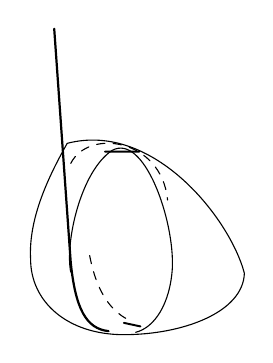
\begin{tikzpicture}[x=0.015cm,y=-0.015cm,line cap=round,line join=round,inner sep=0.4pt]
\draw (46,30)..controls(119,11)and(184,94)..(196,140)..controls(195,173)and(144,192)..(94,192)..controls(46,192)and(15,164)..(15,128)..controls(13,92)and(32,55)..(46,30);
\draw[thick] (35,-67)--(49,131)..controls(53,170)and(62,187)..(81,189);
\draw (49,139)..controls(44,115)and(57,54)..(84,36)..controls(111,21)and(137,95)..(135,136)..controls(133,166)and(120,186)..(104,190);
\draw[dashed] (49,47)..controls(64,17)and(126,26)..(131,78) (65,125)..controls(70,151)and(80,171)..(99,180);
\draw[line width=.7pt] (78,37)--(107,37) (94,182)--(108,185);

\end{tikzpicture}}

$\Sigma$ est une partie ouverte de $E$ i.e. $\alpha\in\Sigma$, $\beta\in E$, $\beta>\alpha$ implique $\beta\in\Sigma$. Donc dans $\Sigma$ comme dans $E$, tte partie majorée a un Sup (car c'est le cas \deleted{dans} $\mathbb F_3$) \inserted{de m} \deleted{\unsure{tout|toute}} partie minorée de $\Sigma$ a un Inf.
\scanpage{21}
% archive sheet number: 20

\figure{\begin{tikzpicture}[x=.00555cm,y=-.00555cm,line cap=round,line join=round,inner sep=.4pt]
% Drawing 1
\begin{scope}
\draw (54,274)--(329,81) (57,244)--(380,117) (149,82)--(344,285) (233,34)..controls(269,133)and(300,228)..(331,358);
\draw (527,62)--(525,515) (538,62)..controls(551,156)and(534,382)..(541,530);
\node[scale=0.8,transform shape=false] at (176,357) {$4$};
\node[scale=0.7,transform shape=false] at (327,418) {$(\mathfrak S_{\unsure{4|1}})$};
\node[scale=0.75,transform shape=false] at (196,519) {$(1)$};
\end{scope}
% Drawing 2
\begin{scope}
\draw (628,297)--(982,131) (694,284)--(921,87) (692,135)..controls(807,134)and(954,168)..(1064,171) (762,105)..controls(791,86)and(863,211)..(992,334) (844,56)..controls(870,151)and(972,336)..(1005,442);
\node[scale=0.72,transform shape=false] at (828,361) {$5\ \mathrm{pos.}$};
\node[scale=0.68,transform shape=false] at (775,427) {$(D_5)\quad\text{générale}$};
\node[scale=0.52,transform shape=false] at (1093,477) {$\deleted{\unsure{\mathfrak S_5^{*}}}$};
\node[scale=0.72,transform shape=false] at (848,555) {$(2)$};
\end{scope}
% Drawing 3
\begin{scope}
\draw (1200,285)--(1555,110) (1226,291)--(1482,53) (1331,331)..controls(1377,247)and(1429,113)..(1472,27) (1372,49)--(1497,325) (1424,29)--(1513,407);
\node[scale=0.7,transform shape=false] at (1382,399) {$5\ \text{position}$};
\node[scale=0.7,transform shape=false] at (1385,475) {$\text{particulière}$};
\node[scale=0.72,transform shape=false] at (1358,574) {$(3)$};
\end{scope}
% Drawing 4
\begin{scope}
\draw (1729,316)..controls(1852,313)and(1990,297)..(2139,290) (1732,353)--(2096,159) (1760,361)--(1973,112) (1816,183)--(2145,343) (1922,93)--(2101,390) (1935,355)..controls(1946,283)and(1944,153)..(1956,87);
\foreach \x/\y in {1807/311,1945/236,1953/134,2052/295}{\fill (\x,\y) circle (7);}
\node[scale=0.7,transform shape=false] at (2016,406) {$6\ \text{en position}$};
\node[scale=0.69,transform shape=false] at (2030,457) {$\text{\unsure{tétraédrale|tétraèdrale}}$};
\node[scale=0.72,transform shape=false] at (1930,519) {$(4)$};
\end{scope}

\end{tikzpicture}}

Tout arrangement 1-dim. de ps. droites \deleted{qui \unsure{est un}} \deleted{\unsure{contient}} \unsure{provenant|pouvant|comportant} \deleted{\unsure{plan|des|être}} de ps. droites bigonal, \deleted{contient une des $4$ configurations} \inserted{si elle n'est réduit à $4$ ps droites (auquel cas c'est le cas (1))} contient une des \inserted{types de} configurations (2) (3) (4) qui sont \deleted{``spéciales'', \unsure{soit}} ``non spéciales'', i.e. quand elles sont réalisées par des arrangements \inserted{2-dim.} de ps. droites, alors l'intersection de deux faces fermées est \deleted{une face,} vide, réduite à un sommet, ou est une arête fermée.

\uline{NB} Si elle ne contient (2) ni (3), alors \deleted{c'est} elle est du type (4), ou du type (5)

\figure{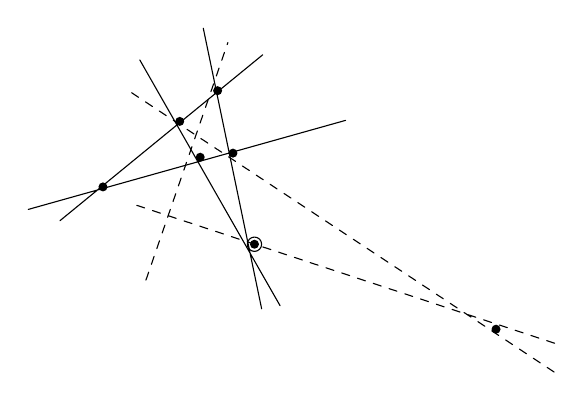
\begin{tikzpicture}[x=0.013cm,y=-0.013cm,line cap=round,line join=round,inner sep=0.4pt]
\draw (1111,1433)--(1421,1346) (1142,1444)--(1340,1282) (1220,1287)--(1357,1527) (1282,1256)--(1339,1530);
\draw[dashed] (1212,1319)--(1628,1594) (1226,1502)--(1306,1270) (1217,1429)--(1626,1564);
\foreach \x/\y in {1184/1411,1259/1347,1296/1317,1279/1382,1311/1378,1332/1467,1568/1550}{\fill (\x,\y) circle (4.4);}
\draw (1332,1467) circle (7);

\end{tikzpicture}}

de $7$ ps. droites formé d'un quadrilatère et de trois diagonales, qui mérite d'être étudié

\deleted{Si elle ne contient}
